\documentclass[twoside]{article}

\usepackage[a4paper, total={674pt, 426pt}, landscape]{geometry}
\usepackage{multicol}

\newcommand{\todo}[1]{\textcolor{red}{\textbf{TODO:} #1}}
\newcommand{\dyade}[1]{\overleftrightarrow{#1}}
\newenvironment{definition}[1]{\begin{tcolorbox}[title=Def.: #1, colback=white!,colframe=green!50!black]}{\end{tcolorbox}}

\titlespacing*{\section}{0pt}{.6\baselineskip}{.1\baselineskip}
\titlespacing*{\subsection}{0pt}{.6\baselineskip}{.1\baselineskip}
\titlespacing*{\subsubsection}{0pt}{.6\baselineskip}{.1\baselineskip}


%% This is the space for custom commands for your Formelsammlung
\newcommand{\FormelsammlungTitel}{Baulelemente der Mikro- und Leistungselektronik}
\newcommand{\FormelsammlungAutor}{Bogdan Stamenic}
\setcounter{tocdepth}{2} % Show only sections and subsection in table of contents

\begin{document}
	\title{\FormelsammlungTitel}
	\author{\FormelsammlungAutor}
	\date{\today}
	\begin{multicols*}{2}
%		\begin{minipage}{.4\paperheight}
			\maketitle
			\tableofcontents
        % \end{minipage}
        \section{Introduction}
\subsection{Example Applications of Semiconductor Power Electronics}
\begin{itemize}
        \item RF Transmission
        \item Welding Generators
        \item Uninterruptible Power Supply (UPC)
        \item Buck-/Boost-Wandler
        \item Wechselrichter (Power Inverter)
\end{itemize}
\subsection{Semiconductor Microsensor, -actuators and -systems}
\begin{itemize}
    \item Wandler (Transducer) wandeln nicht-elek. in elek. Energie um bzw. umgekehrt
    \item Pressure Sensor
        \begin{itemize}
            \item Determine altitude by measuring pressure
            \item $p(\Delta h) = p(h_{0}) \exp\left(-\dfrac{\Delta h}{h_{s}}\right)$
            \item Determine altitude and, hence floor inside a building (indoor navigation)
        \end{itemize}
    \item Micromechanical Mass Air Flow Meter
        \begin{itemize}
            \item heater and two pairs of resistive temperature sensors, placed on micromachined bridge
            \item heater provides temperature profile on thermally insulated bridge
            \item without mass flow: symmetric temperature profile
            \item with mass flow: temperature profile distorted
            \item temperature difference $\Delta T$ is measure for mass flow
        \end{itemize}
\end{itemize}
\begin{tabularx}{.5\textwidth}{XX}
    \toprule
    CMOS-Circuits/ICs & Semiconductor Sensors\\
    \midrule
    flat, small structure height ($\mu m$) & Larger feature size, depth/height up to wafer thickness ($~300 - \SI{800}{\mu m}$)\\
    \midrule
    no mechanically movable parts & mechanically movable parts, cavities, alternative materials $\to$ additional fabrication processes needed\\
    \midrule
    Functionality by internal processes in bulk (carrier transport)  & Sensor effect typicall at the surface (contact to environment)\\
    \midrule
    Complete protection of dies against environmental impact on wafer level & Structures typically exposed\\
    \midrule
    Standardized packaging technology possible & Larger variety of individual packaging solutions\\
    \bottomrule
\end{tabularx}

        \section{Physical Fundamentals}
\subsection{Electronic Transport}
\subsubsection{Drude Model}
\begin{itemize}
  \item Electric field applied to conducting material accelerates carriers
  \item Carriers are scattered by impurities and lattice atoms
        \begin{align*}
          &\vec{v}_{D} = \mu \vec{E} &\text{: mean drift velocity},\\
          &\vec{j} = en\vec{v}_{D} &\text{: elec. current density},\\
          \implies&\vec{j} = \underbrace{en\mu}_{\sigma} \vec{E} = \sigma_{n} \vec{E}
        \end{align*}
  \item Two carrier species in semiconducting materials: electrons and holes
  \item Driving force of drift current is electric potential $\varphi$
        \begin{align*}
          &\vec{j_{n}}(\vec{r}) = en\mu_{n}\vec{E} = \sigma_{n}\vec{E} = -\sigma_{n}\nabla\varphi,\\
          &\vec{j_{p}}(\vec{r}) = en\mu_{p}\vec{E} = \sigma_{p}\vec{E} = -\sigma_{p}\nabla\varphi
        \end{align*}
        \item Additional driving force in semiconductors is gradient of carrier concentration
        \begin{align*}
          &\vec{j}_{n}(\vec{r}) = eD_{n}\nabla n,\\
          &\vec{j}_{p}(\vec{r}) = eD_{p}\nabla p,\\
          &D_{n,p} = \dfrac{kT}{q}\mu_{n,p} & \text{: Einstein's relation}
        \end{align*}
  \item \textbf{Drift-diffusion} model for electrons and holes
        \begin{align*}
          &\vec{j}_{n}(\vec{r}) = en\mu_{n}\vec{E} + \mu_{n}kT\nabla n\\
          &\vec{j}_{p}(\vec{r}) = \underbrace{en\mu_{p}\vec{E}}_{\text{drift current}}
          + \underbrace{\mu_{p}kT\nabla p}_{\text{diffusion current}}
        \end{align*}
\end{itemize}

\subsubsection{Continuity Equations}
\begin{align*}
  \dfrac{\partial n}{\partial t} = \dfrac{1}{e} \mathrm{div}\,\vec{j}_{n}(\vec{r}) + G - R + \dfrac{\partial N_{D}^{+}}{\partial t}\\
  \dfrac{\partial p}{\partial t} = \dfrac{1}{e} \mathrm{div}\,\vec{j}_{p}(\vec{r}) + G - R + \dfrac{\partial N_{A}^{-}}{\partial t}\\
\end{align*}

\subsection{Structure of Matter}
\begin{itemize}
  \item Energie levels of free particals can be described by a parabols $E = f(p^{2}, k^{2})$ in $k$-space.
        \begin{equation*}
          E = \dfrac{p^{2}}{2m} = \dfrac{\hbar^{2}\cdot k^{2}}{2m}
        \end{equation*}
  \item Parabolic Approximation: locally at minima and maxima for energy bands
\end{itemize}

\begin{definition}{Density of States $N_{n,p}(E)$ (Zustandsdichte)}
  The number (or density) of states per energy intervall $\mathrm{d}E$. Useful for calculating the number of carriers $n$ or $p$.

  For parabolic bands:
  \begin{align*}
    N_{n}(E) \, \mathrm{d}E = \dfrac{2\pi \cdot {(2m_{n}^{*})}^{3/2}}{h^{3}} \sqrt{E - E_{c}} \, \mathrm{d}E\\
    N_{p}(E) \, \mathrm{d}E = \dfrac{2\pi \cdot {(2m_{p}^{*})}^{3/2}}{h^{3}} \sqrt{E_{v} - E} \, \mathrm{d}E\\
  \end{align*}
\end{definition}

\begin{itemize}
  \item Fermi-Dirac distribution describes electron (fermion) distribution
        \begin{equation*}
          f_{\mathrm{FD}}(E) = \dfrac{1}{1 + \exp \left(\dfrac{1}{kT} (E - E_{F})\right)}
        \end{equation*}
  \item For parabolic bands:
        \begin{equation*}
          f_{\mathrm{FD}}(E) \approx \exp \left(- \dfrac{E_{\mathrm{gap}}}{2 kT}\right)
        \end{equation*}
  \item $n(T)$ and $p(T)$ determined by integrating over the respective energy space:
        \begin{equation*}
        n(T) = \int N_{n}(E)f(T, E) \, \mathrm{d}E
        \end{equation*}
  \item Mass action law for carrier concentration (also for doped semiconducters)
        \begin{equation*}
          n_{i}^{2} = n \cdot p
        \end{equation*}
\end{itemize}

\subsection{Charateristic Properties of Semiconductors}
\begin{itemize}
  \item Electric conductivity depends on carrier number $n$ or $p$ and mobility $\mu$
        \begin{equation*}
          \sigma_{\alpha} = e\alpha \mu_{\alpha}, \quad \alpha = n, p
        \end{equation*}
  \item Carrier mobility:
        \begin{align*}
          \mu_{\alpha} := \dfrac{|\vec{v}_{\alpha}|}{|\vec{E}|} = e \dfrac{\tau_{\alpha}}{m_{\alpha}}, \quad \alpha = n, p, \quad [\mu] = \dfrac{\si{cm^{2}}}{\si{Vs}}
        \end{align*}
  \item Carrier mobility depends on
        \begin{itemize}
                \item Temperature $\mu \propto T^{\beta}$ with $\beta \approx \begin{cases}+3/2, \quad \text{for low T (impurity scattering)}\\ -3/2, \quad \text{for high T (phonon scattering)} \end{cases}$
                \item Doping concentration: scattering throught ionized impurities reduces $\tau_{\alpha}$
        \end{itemize}
        \begin{tabular}{cc}
          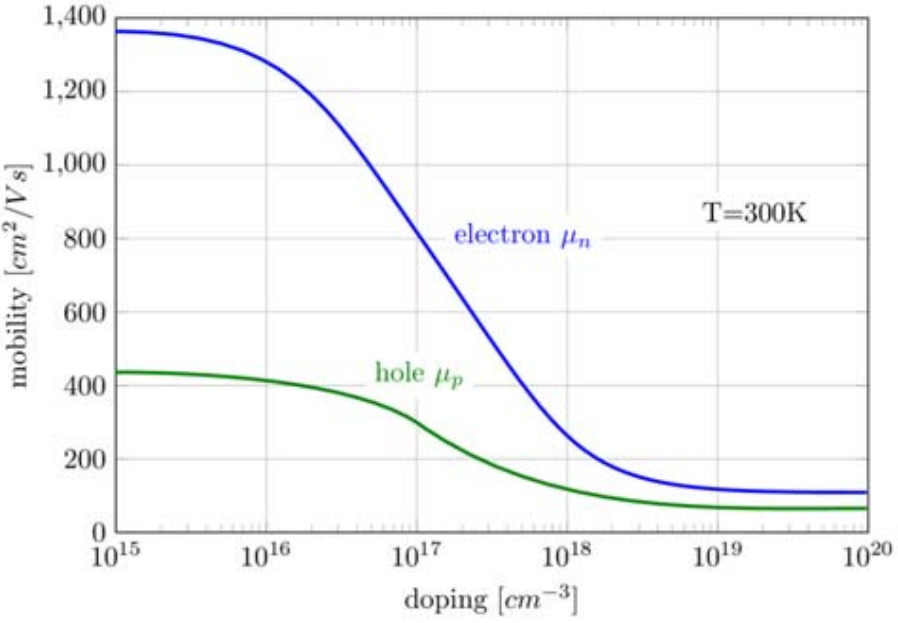
\includegraphics[width=.25\textwidth]{content/bdml/pictures/electron_vs_hole_mobility}
          &
          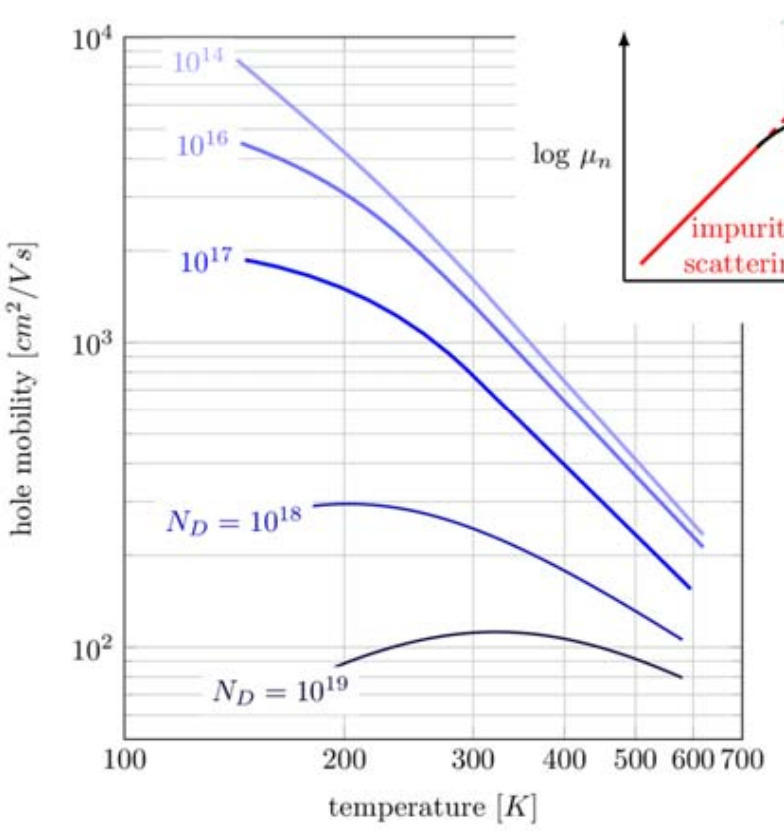
\includegraphics[width=.22\textwidth]{content/bdml/pictures/hole_mobility_doping}
        \end{tabular}
  \item Scattering of carriers:
        \begin{enumerate}
          \item impurity scattering (doping dependence)
          \item phonon scattering (temperature dependence)
          \item carrier-carrier scattering
        \end{enumerate}
        \item Drift velocity $\vec{v}_{D}$ saturates for high $\vec{E}$ $\implies$ $\lim\limits_{\vec{E} \to \infty} \vec{v}_{D} = const$
  \item Elec. conductivity
        \begin{equation*}
          \sigma = \dfrac{1}{\rho} = q \, (n\mu_{n} + p\mu_{p})
        \end{equation*}
  \item Thermal heat flow:
        \begin{equation*}
          \vec{J}_{Q} = -\kappa \, \nabla T
        \end{equation*}
  \item Elec. and thermal conductivity related by \textbf{Wiedemann-Franz} law:
        \begin{equation*}
          \dfrac{\kappa_{n}}{\sigma_{n}} = L \, T, \quad L = \begin{cases} \dfrac{1}{3}{\left(\dfrac{\pi k_{B}}{e}\right)}^{2} \quad \text{metal}\\ 2{\left(\dfrac{k_{B}}{e}\right)}^{2} \quad \text{semiconducter} \end{cases}
        \end{equation*}
\end{itemize}

        \section{Basic Semiconductor Device Structures}
\subsection{pn Junction --- pn Diode}
\begin{itemize}
        \item Carriers recombine and a \textbf{space charge region} (SCR) with an elec. field $\vec{E}$ arises
  \item At thermal equilibrium:
        \begin{align*}
          &\vec{j}_{n, \mathrm{drift}} = \vec{j}_{n, \mathrm{diff}}\\
          &\vec{j}_{n}(\vec{r}) = en\mu_{n}\vec{E} + \mu_{n}kT\,\nabla n = 0\\
          &\vec{j}_{p}(\vec{r}) = en\mu_{p}\vec{E} - \mu_{p}kT\,\nabla p = 0
        \end{align*}
\end{itemize}

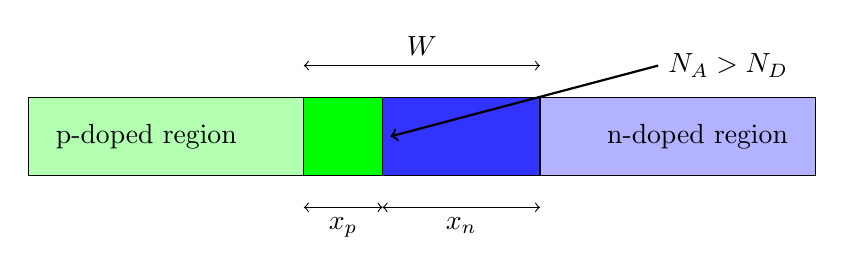
\begin{tikzpicture}
  \pgfmathsetmacro{\pnJunction}{4.5};
  \pgfmathsetmacro{\scrLeft}{3.5};
  \pgfmathsetmacro{\scrRight}{6.5};
  %% Semiconductor blocks
  \filldraw[draw=black!, fill=green!30] (0,0) rectangle (\pnJunction,1);
  \filldraw[draw=black!, fill=blue!30] (\pnJunction,0) rectangle (10,1);
  \draw (1.5,.5) node[]{p-doped region};
  \draw (8.5,.5) node[]{n-doped region};
  %% Space Charge Region (SCR)
  \filldraw[draw=black!, fill=green!] (\scrLeft,0) rectangle (\pnJunction,1);
  \filldraw[draw=black!, fill=blue!80] (\pnJunction,0) rectangle (\scrRight,1);
  %% Measurements
  \draw[<->] (\scrLeft, 1.4) -- node[above]{$W$} (\scrRight, 1.4);
  \draw[<->] (\scrLeft, -.4) -- node[below]{$x_{p}$} (\pnJunction, -.4);
  \draw[<->] (\pnJunction, -.4) -- node[below]{$x_{n}$} (\scrRight, -.4);
  %% Label
  \draw[->, thick] (8, 1.4) node[right]{$N_{A} > N_{D}$} -- (\pnJunction + .1, .5);
\end{tikzpicture}

\begin{align*}
  &x_{p} \cdot N_{A} = x_{n} \cdot N_{D} & \text{: charge neutrality}\\
  &W = x_{p} + x_{n} & \text{: width of depletion region}
\end{align*}

\begin{itemize}
        \item Abrupt pn junctions block more voltage
\end{itemize}

\subsection{Metal-Semiconductor Junctions}
\begin{itemize}
  \item Application as diodes with low threshold voltage and ohmic contacts
  \item Properties of Schottky diodes:
        \begin{itemize}
          \item current carried by majority carriers
          \item $V_{th}$ lower than in pn diodes
          \item fast switching time (application in fast logic and HF circuits)
          \item \textcolor{red}{But:} higher reverse current and lower blocking capability
        \end{itemize}
  \item Schottky diodes as freewheeling diodes (low junction voltage)
  \item Schottky diodes with wide-bandgap materials for better blocking
        \begin{equation*}
          j = j_{s} \cdot \left(\exp\left[\dfrac{qV_{f}}{kT}\right] - 1\right), \quad j_{s} = \underbrace{A^{*}}_{\text{Richardson const.}}\, T^{2} \exp\left(\dfrac{-q V_{B}}{kT}\right)
        \end{equation*}
    \item For ohmic contacts: highly doped semiconductors are used, creating a thinner barrier $\implies$ tunneling of electron possible
\end{itemize}

\section{Bipolar Transistor}
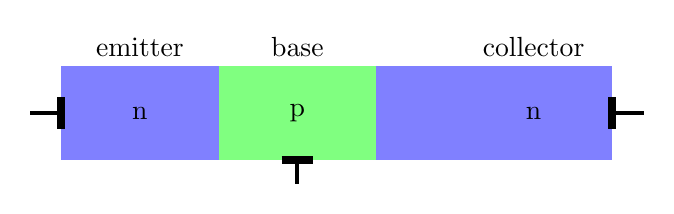
\begin{tikzpicture}
  %% Conveniant macros for adjusting size later
  \pgfmathsetmacro{\blockHeight}{1.2}
  \pgfmathsetmacro{\blockLength}{7}
  \pgfmathsetmacro{\emitterBaseJunction}{2}
  \pgfmathsetmacro{\baseCollectorJunction}{4}
  \pgfmathsetmacro{\baseMiddle}{(\emitterBaseJunction + \baseCollectorJunction) / 2}
  %% npn-blocks
  \fill[fill=blue!50] (0,0) rectangle (\emitterBaseJunction, \blockHeight);
  \fill[fill=green!50] (\emitterBaseJunction,0) rectangle (\baseCollectorJunction, \blockHeight);
  \fill[fill=blue!50] (\baseCollectorJunction, 0) rectangle (\blockLength, \blockHeight);
  %% Contacts
  \draw[line width=1mm] (0,\blockHeight / 2 + .2) -- (0,\blockHeight / 2 - .2);
  \draw[line width=.5mm] (0,\blockHeight / 2) -- (-.4,\blockHeight / 2);
  \draw[line width=1mm] (\blockLength,\blockHeight / 2 + .2) -- (\blockLength,\blockHeight / 2 - .2);
  \draw[line width=.5mm] (\blockLength,\blockHeight / 2) -- (\blockLength + .4,\blockHeight / 2);
  \draw[line width=1mm] (\baseMiddle - .2,0) -- (\baseMiddle + .2,0);
  \draw[line width=.5mm] (\baseMiddle,0) -- (\baseMiddle,-.3);
  %% Labels
  \draw (1,\blockHeight) node[above]{emitter};
  \draw (1,\blockHeight / 2) node[]{n};
  \draw (3,\blockHeight) node[above]{base};
  \draw (3,\blockHeight / 2) node[]{p};
  \draw (6,\blockHeight) node[above]{collector};
  \draw (6,\blockHeight / 2) node[]{n};
\end{tikzpicture}
\begin{itemize}
  \item Electrons injected by emitter into base
        \begin{itemize}
                \item partially recombine with holes $\implies$ holes are replaced via base current
                \item $l_{\mathrm{diff}} > w_{b}$: diffusion of electrons into collector region $\implies I_{c}$
        \end{itemize}
        \item Small changes in base current $\implies$ large impact on collector current
\end{itemize}

\section{MOS Structure --- MOS Field Effect Transistor}

	\end{multicols*}
\end{document}
